\documentclass{article}

% NeurIPS 2024 template
\usepackage{neurips_2024}

\usepackage[utf8]{inputenc} % allow utf-8 input
\usepackage[T1]{fontenc}    % use 8-bit T1 fonts
\usepackage{hyperref}       % hyperlinks
\usepackage{url}            % simple URL typesetting
\usepackage{booktabs}       % professional-quality tables
\usepackage{amsfonts}       % blackboard math symbols
\usepackage{nicefrac}       % compact symbols for 1/2, etc.
\usepackage{microtype}      % microtypography
\usepackage{xcolor}         % colors
\usepackage{amsmath}        % mathematical expressions
\usepackage{graphicx}       % graphics support

\usepackage{threeparttable} % table notes for self-contained captions


\title{Scaling Environments for Code Generation Agents: A Production Framework for Agentic Prompt-to-App Generation}

\author{%
  Anonymous Authors \\
  Anonymous Institution \\
  \texttt{anonymous@example.com} \\
}

\begin{document}

\maketitle

\begin{abstract}
We present app.build, an open-source framework that improves LLM-based application generation through systematic validation and structured environments. Our approach combines multi-layered validation pipelines, stack-specific orchestration, and model-agnostic architecture across three reference stacks. Through evaluation on 30 generation tasks, we demonstrate 73.3\% viability with 30\% reaching perfect quality scores, while open-weights models achieve 80.8\% of closed-model performance when provided structured environments. The framework has generated over 3,000 applications, demonstrating that scaling reliable AI agents requires scaling environments, not just models.
\end{abstract}

\section{Introduction}
\label{sec:intro}

\subsection{The Production Reliability Gap}

While AI coding agents demonstrate impressive capabilities on benchmarks like HumanEval \citep{chen2021evaluating} and MBPP \citep{austin2021program}, building production-ready applications without human supervision remains infeasible. Recent systems such as Devin \citep{cognition2024swe} and SWE-agent \citep{yang2024swe} represent significant advances, yet reveal a substantial gap between research benchmarks and production requirements.

This gap manifests across multiple dimensions. Function-level benchmarks like HumanEval evaluate isolated code generation but fail to capture system-level concerns including error handling, integration complexity, and production constraints \citep{liu2023your}. Even state-of-the-art systems like AutoCodeRover, achieving 19\% efficacy on SWE-bench at \$0.43 per issue \citep{zhang2024autocoder}, demonstrate that raw model capability alone is insufficient for reliable automated software development.

The core challenge lies in treating LLMs as standalone systems rather than components requiring structured environments. Current approaches focus on making models ``smarter'' via training or prompt engineering, but fail to address fundamental reliability issues in probabilistic generation. The field requires a shift from model-centric to environment-centric design \citep{jiang2024survey,paul2024benchmarks}.

\subsection{Our Approach: Environment Scaffolding}

\textbf{Definition.} We define \emph{environment scaffolding (ES)} as an environment-first paradigm where the model operates inside a structured sandbox that constrains actions and provides continuous, deterministic feedback. Rather than relying on larger models or prompt-only techniques, ES improves the context around the model---shaping the action space, providing templates and tools, and validating each step---channeling creativity into safe, verifiable outcomes.

\paragraph{Principles.}
\begin{enumerate}
  \item \textbf{Structured task decomposition.} The agent works through an explicit sequence of well-scoped tasks (e.g., schema $\rightarrow$ API $\rightarrow$ UI), each with clear inputs/outputs and acceptance rules.
  \item \textbf{Multi-layered validation.} Deterministic checks (linters, type-checkers, unit/smoke tests, runtime logs) run \emph{after every significant generation}, catching errors early and feeding them back for automatic repair.
  \item \textbf{Runtime isolation.} All code executes in isolated sandboxes (containers) with ephemeral state, enabling safe trial-and-error and reproducible re-runs.
  \item \textbf{Model-agnostic integration.} The scaffolding is decoupled from any particular LLM; different backends can be swapped without changing the workflow.
\end{enumerate}

\paragraph{Why ES vs.\ model-centric approaches?}
Traditional systems prompt an LLM to generate the full solution in one or few passes, with checks (if any) at the end. ES enforces a guarded, iterative loop: generate $\rightarrow$ validate $\rightarrow$ repair, per sub-task. Figure~\ref{fig:es-vs-model} and Table~\ref{tab:es-contrast} summarize the contrast.

\begin{figure}[t]
  \centering
  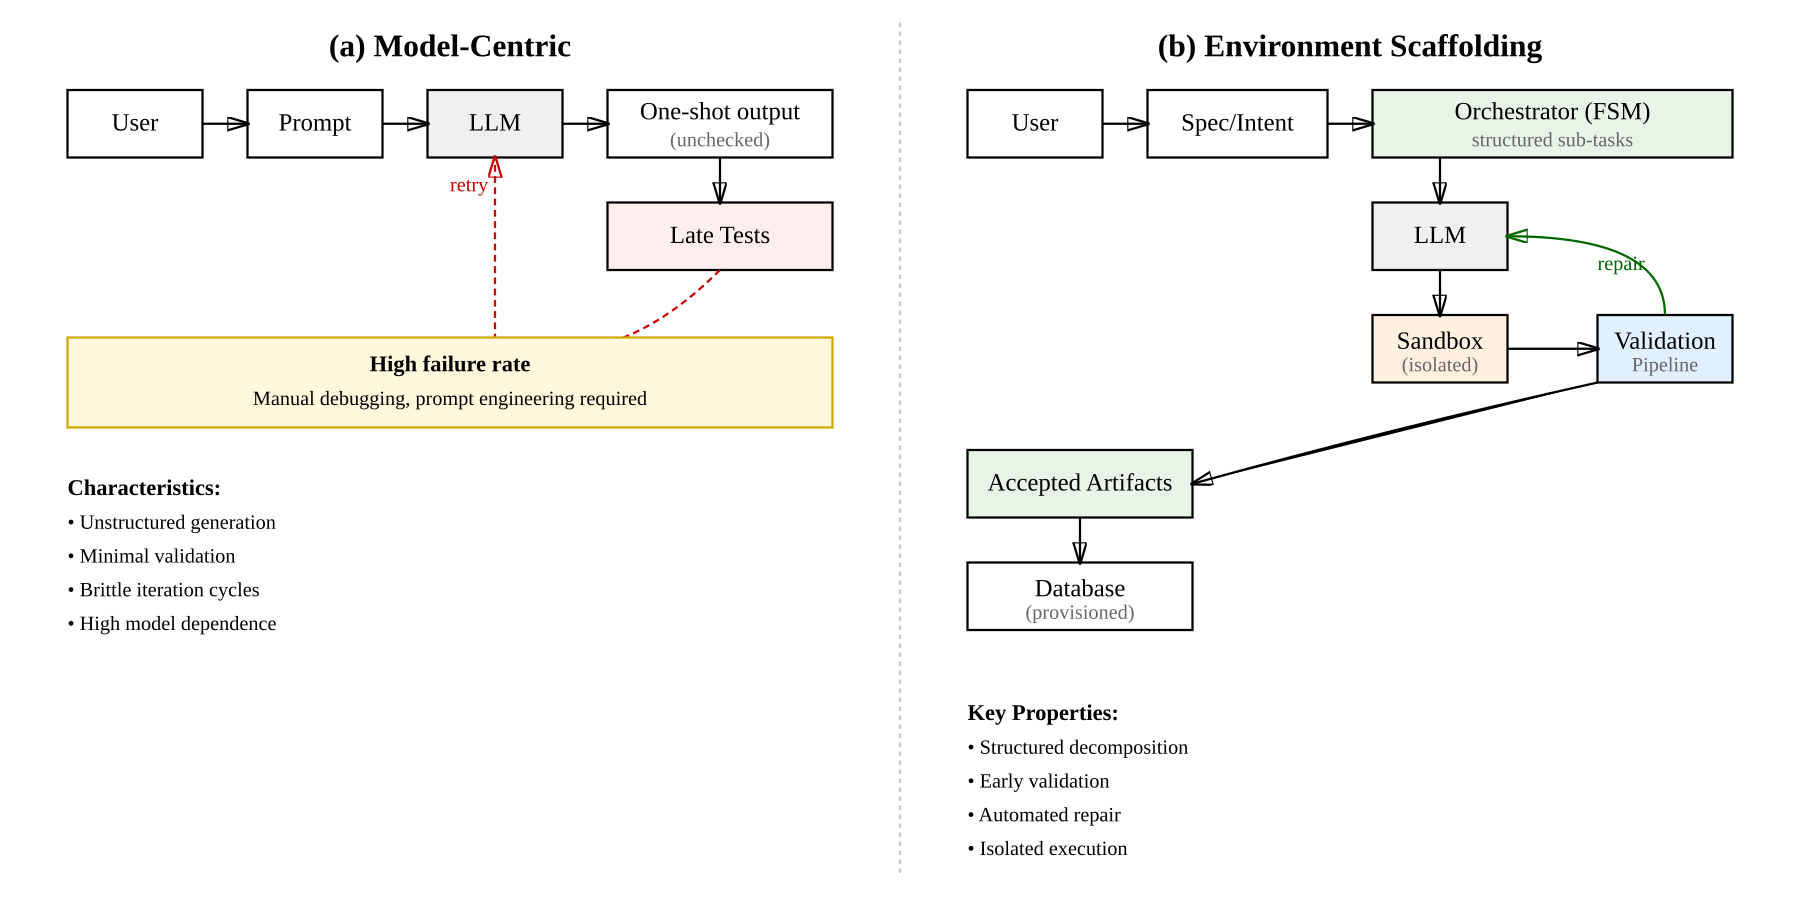
\includegraphics[width=\linewidth]{diagrams/es-vs-model.png}
  \vspace{-0.5em}
  \caption{\textbf{Environment scaffolding vs.\ model-centric generation.} ES wraps the model with a finite, validated workflow that catches errors early and repairs them before proceeding.}
  \label{fig:es-vs-model}
\end{figure}

\begin{table}[t]
\centering
\small
\begin{threeparttable}
\caption{\textbf{Environment scaffolding (ES) vs.\ model-centric generation.}}
\label{tab:es-contrast}
\begin{tabular}{@{}p{3.2cm}p{5.6cm}p{5.6cm}@{}}
\toprule
\textbf{Aspect} & \textbf{Model-Centric} & \textbf{Environment Scaffolding (Ours)} \\
\midrule
Task decomposition & Single/loosely guided multi-step; no fixed structure &
Explicit pipeline (FSM): schema $\rightarrow$ API $\rightarrow$ UI \\
Validation & Late or ad-hoc checks &
Integrated per-step: linters, type checks, unit/smoke tests \\
Error recovery & Manual/ad-hoc retries &
Automatic repair loop using error feedback \\
Execution isolation & Often none; runs on host &
Isolated containers; reproducible runs \\
Model dependence & Strong (prompt/model specific) &
Model-agnostic; environment guides behavior \\
Observability & Limited, coarse logs &
Per-step metrics, artifacts, and logs \\
\bottomrule
\end{tabular}
\end{threeparttable}
\end{table}

\subsection{Contributions}

Our main contributions are:

\begin{itemize}
  \item \textbf{Environment Scaffolding Paradigm.} We formalize environment scaffolding (ES) and show how structuring the action space with per-step validation enables reliable code generation.
  \item \textbf{Open-Source Framework.} We release app.build, implementing ES across three stacks with validators and deployment hooks.\footnote{See repository overview for supported stacks and validators.}
  \item \textbf{Empirical Evaluation.} We quantify validation layer effects and compare multiple LLM backends under the same environment.
  \item \textbf{Methodological Insight.} Improving the environment often matters more than scaling the model for production reliability.
  \item \textbf{Community Adoption.} The framework has generated thousands of applications, demonstrating practical utility.
\end{itemize}

\section{Background and Related Work}
\label{sec:related}

\subsection{Agentic Software Engineering}

AI coding agents have evolved from simple code completion to autonomous software engineering systems. \textbf{SWE-bench} \citep{jimenez2024swe} established the standard for repository-level evaluation with 2,294 real GitHub issues. \textbf{SWE-agent} \citep{yang2024swe} demonstrated that custom agent-computer interfaces significantly enhance performance, achieving 12.5\% pass@1 through interface design rather than model improvements.

\textbf{WebArena} \citep{zhou2024webarena} revealed GPT-4 achieves only 14.41\% success versus 78.24\% human performance, demonstrating that environment design matters more than model capability. \textbf{AutoCodeRover} \citep{zhang2024autocoder} combines LLMs with fault localization, achieving 19\% efficacy on SWE-bench at \$0.43 per issue. \textbf{Agentless} \citep{xia2024agentless} achieved 32\% on SWE-bench Lite with a simple three-phase process, suggesting sophisticated architectures may not always improve performance.

\textbf{Multi-agent systems} consistently outperform single-agent approaches. \textbf{AgentCoder} \citep{huang2023agentcoder} employs three agents (Programmer, Test Designer, Test Executor) achieving 96.3\% pass@1 on HumanEval versus 71.3\% for single-agent approaches. \textbf{MetaGPT} \citep{hong2023metagpt} demonstrates role-based agents achieving 85.9\% pass@1 on HumanEval with 100\% task completion.

\subsection{Production Quality in Generated Code}

Production-ready AI-generated code requires validation beyond simple correctness testing. Static analysis integration reduces false-positive rates from 85\% to 66\%. Test-driven approaches like TiCoder achieve 45.97\% absolute improvement through interactive generation. Property-based testing shows 23.1--37.3\% relative improvements by capturing semantic properties rather than specific implementations.

AST-based validation provides structural correctness guarantees, with AST-T5 outperforming CodeT5 by 2--3 points. Industry deployment reveals gaps between offline performance and practical usage, as evidenced by CodeAssist's analysis of 2M completions from 1,200+ users.

\subsection{Tree Search}

Tree search enhances LLM-based solutions by increasing compute budget beyond internal model reasoning. Li et al.'s S* Scaling \citep{li2025s} combines iterative feedback with parallel branches. Sampling more trajectories increases success rates significantly, with pass@1 and pass@3 often differing by 30\% or more.

\subsection{Runtime Isolation and Scaling}
Sandboxing is essential for web applications requiring elaborate testing including database setup and browser emulation. We use Dagger.io for parallel scaling with caching and Docker compatibility.

\section{Problem Setup and Method}
\label{sec:method}

\subsection{Problem Formulation}

LLM-based code generation enables rapid prototyping but often fails production standards. We formalize this as an environment design problem where success depends on structured constraints and validation feedback, not just model capability.

\begin{figure}[t]
  \centering
  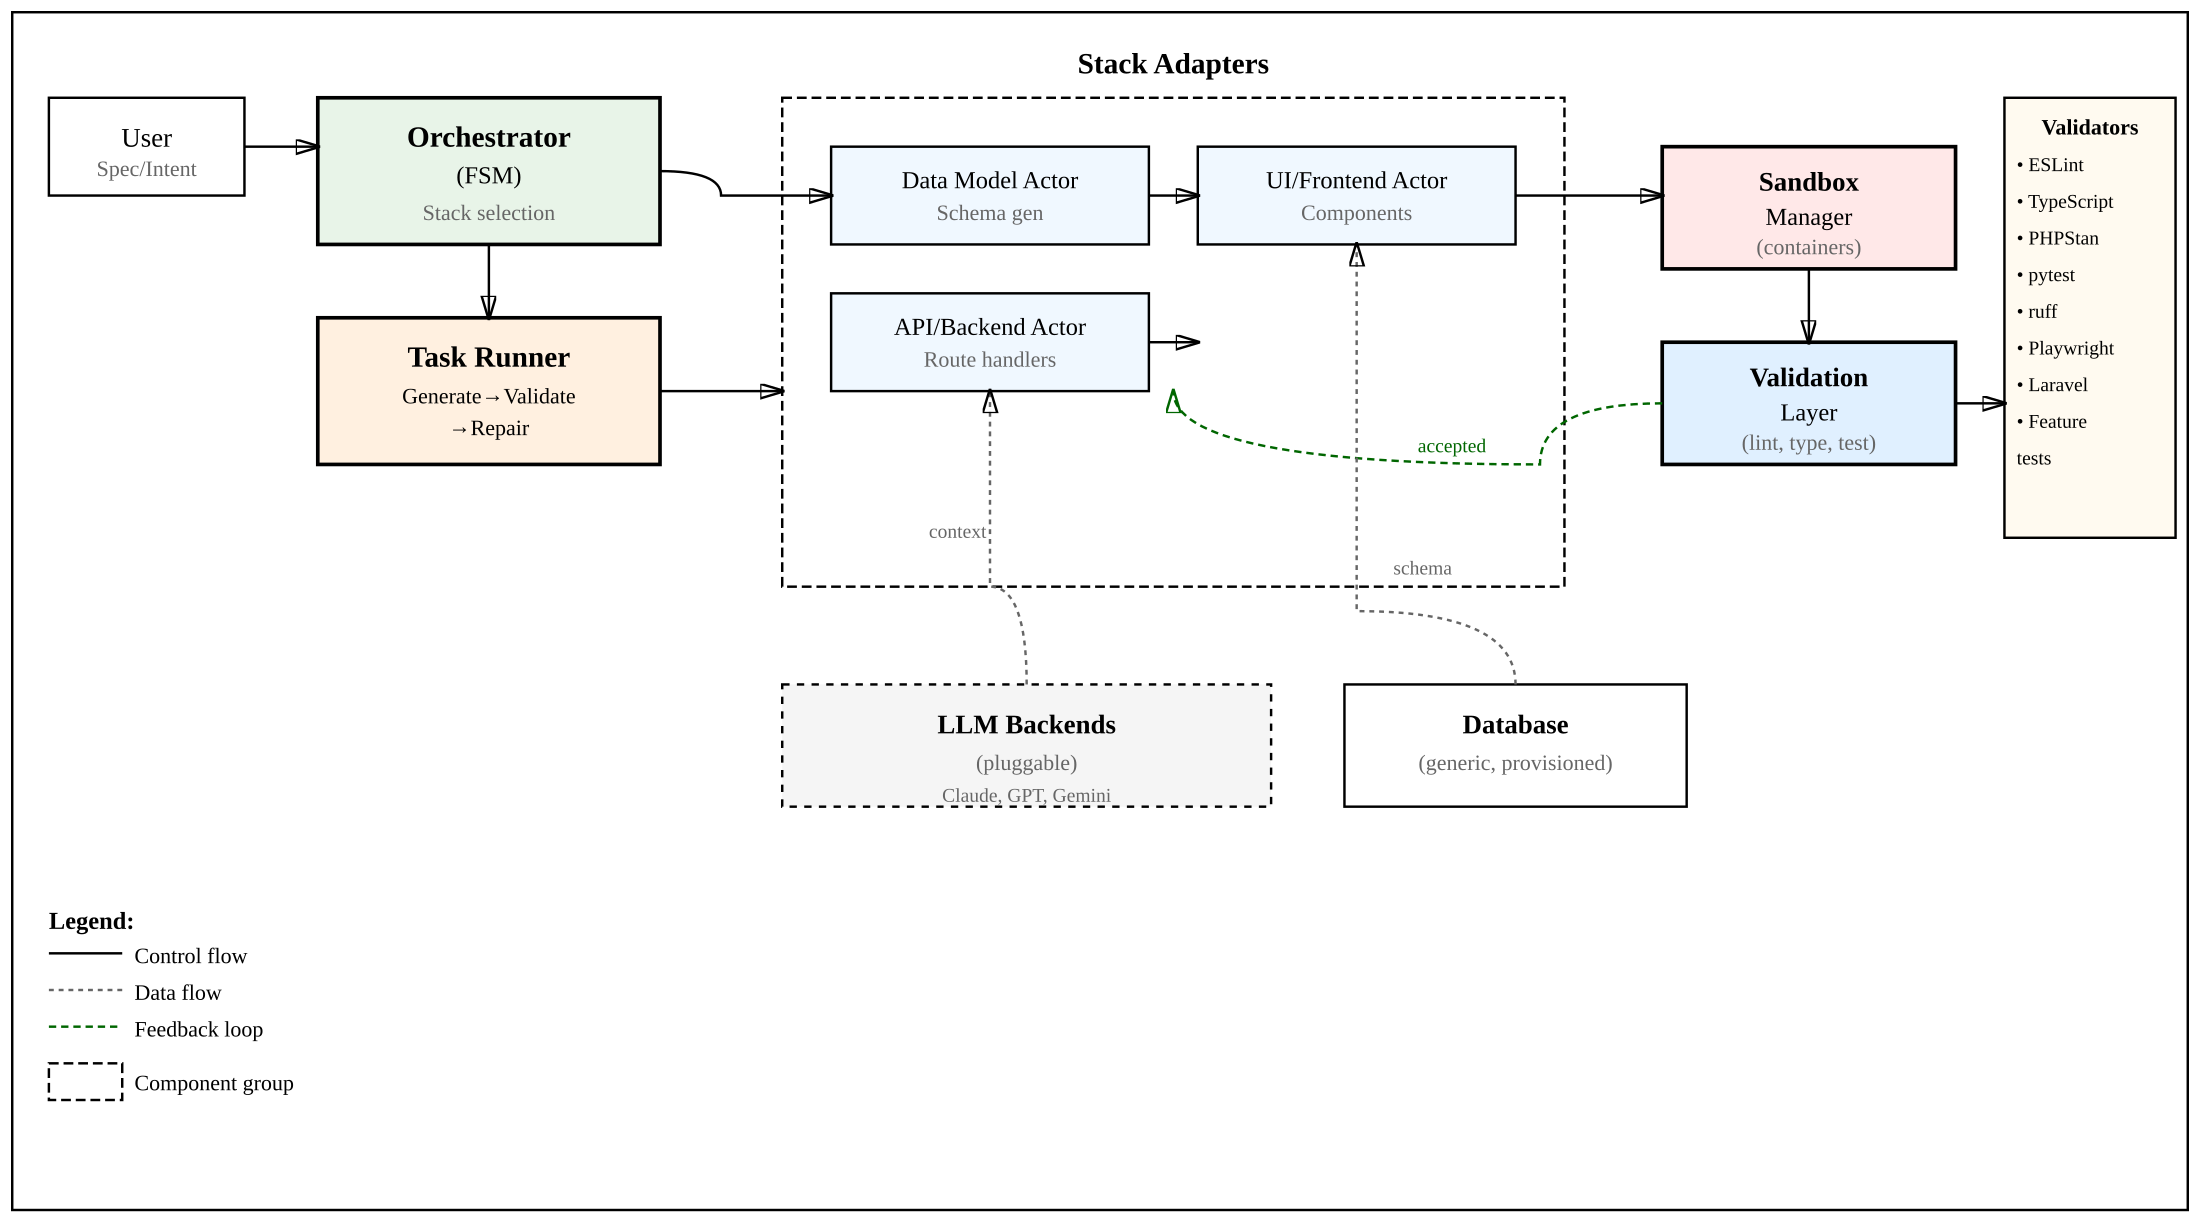
\includegraphics[width=\linewidth]{diagrams/appbuild-arch.png}
  \vspace{-0.5em}
  \caption{\textbf{app.build architecture} expressed through environment scaffolding. The orchestrator plans stages per stack; each sub-task runs in a sandbox, is validated, and only then merged. CI/CD and DB provisioning are integrated.}
  \label{fig:appbuild-arch}
\end{figure}

\subsection{Architecture}

\textbf{High-level design.} The app.build agent implements ES with a central orchestrator that decomposes specifications into stack-specific stages, executing each in an isolated sandbox with validation before acceptance. The workflow applies across three stacks (TypeScript/tRPC, PHP/Laravel, Python/NiceGUI) with stack-aware validators and managed Postgres databases.

\textbf{Execution loop.} For each sub-task, the agent assembles context, prompts the LLM, executes results in a sandbox, collects validator feedback, and either accepts or repairs the artifact. This iterative loop provides model-agnostic robustness and scales through parallelized sandboxes.

\section{Experimental Setup}
\label{sec:experimental-setup}

We designed experiments using a custom prompt dataset and metrics to evaluate viability and quality of generated applications.

\subsection{Evaluation Framework}

\subsection{Prompt Dataset}
\label{sec:prompt-dataset-desc}

The evaluation dataset comprises 30 prompts created by independent contributors reflecting authentic development workflows. Prompts were filtered to exclude enterprise integrations and capabilities beyond framework scope, then post-processed for anonymization and standardization. The dataset spans three complexity levels: low (static/single-page UI), medium (single-entity CRUD), and high (multi-entity/custom logic).
See the full list of prompts in Appendix~\ref{sec:prompt-dataset}.

\subsection{Metrics}

Each generated application was evaluated using metrics assessing viability and quality under preset constraints.

\begin{itemize}
\item Viability rate ($V=1$) and non-viability rate ($V=0$)
\item Perfect quality rate ($Q=10$) and quality distribution (mean/median for $V=1$ apps)
\item Validation pass rates by check (AB-01, AB-02, AB-03, AB-04, AB-06, AB-07)
\item Quality scores ($Q$, 0--10) using the rubric in Section~\ref{sec:scoring}
\item Model/cost comparisons where applicable
\end{itemize}

\subsection{Experimental Configurations}

We designed three configurations to evaluate factors affecting generation success:

\textbf{Configuration 1: Baseline}. Default tRPC apps with all validation checks enabled.
\textbf{Configuration 2: Model Analysis}. Comparing Claude Sonnet 4 against Qwen3-Coder-480B-A35B \citep{qwen2025qwen3} and GPT OSS 120B \citep{openai2025gpt}.
\textbf{Configuration 3: Validation Ablation}. Three studies isolating validation impact: (3a) disabled Playwright tests; (3b) disabled ESLint; (3c) removed handler tests.

\subsection{Assessor Protocol and Scoring}
\label{sec:scoring}

We implement a structured evaluation protocol with six standardized checks executed by human assessors, reporting binary viability ($V$) and 0--10 quality scores ($Q$).

\textbf{Viability (binary)}:
\begin{equation}
V = \begin{cases}
1 & \text{if AB-01 and AB-02 are not FAIL} \\
0 & \text{otherwise}
\end{cases}
\end{equation}

\textbf{Quality (0--10)}:
\begin{equation}
Q = 10 \times \frac{\sum_{c \in A} w \times s_c}{\sum_{c \in A} w}
\end{equation}

where $A$ is the set of applicable checks (excluding NA) with equal weights, and per-check grades $s_c$ are:
\begin{itemize}
\item AB-01 (Boot): PASS = 1.0, WARN = 0.5, FAIL = 0.0
\item AB-02 (Prompt correspondence): PASS = 1.0, WARN = 0.5, FAIL = 0.0
\item AB-03, AB-04, AB-06 (Clickable Sweep): PASS = 1.0, WARN = 0.5, FAIL = 0.0
\item AB-07 (Performance): continuous metric normalized to $[0,1]$
\end{itemize}

\begin{table}[t]
\caption{Check weights and definitions used in scoring (see rubric in Section~\ref{sec:scoring}). All checks share equal weight after NA re-normalization; AB-01 and AB-02 are hard gates for Viability $V$.}
\label{tab:check-weights}
\centering
\begin{threeparttable}
\begin{tabular}{llcl}
\toprule
Check ID & Check Description & Weight (share) & Notes \\
\midrule
AB-01 & Boot \& Home & 1/6 & Hard gate for Viability $V$ \\
AB-02 & Prompt Correspondence & 1/6 & Hard gate for Viability $V$ \\
AB-03 & Create Functionality & 1/6 &  \\
AB-04 & View/Edit Operations & 1/6 &  \\
AB-06 & Clickable Sweep & 1/6 &  \\
AB-07 & Performance Metrics & 1/6 & Continuous; normalized to $[0,1]$ \\
\bottomrule
\end{tabular}
\begin{tablenotes}
\item \textit{Note.} See mapping of PASS/WARN/FAIL to numeric scores and viability definition in Section~\ref{sec:scoring}.
\end{tablenotes}
\end{threeparttable}
\end{table}

\section{Results}
\label{sec:results}

\subsection{Environment Scaffolding Impact (TypeScript/tRPC only)}

Evaluating 30 TypeScript/tRPC applications, we observe that 73.3\% (22/30) achieved viability ($V=1$), with 30.0\% attaining perfect quality ($Q=10$) and 26.7\% non-viable ($V=0$). Once viability criteria are met, generated applications exhibit consistently high quality.

\begin{table}[t]
\caption{Aggregated evaluation results for TypeScript/tRPC ($n=30$ prompts). Viability $V$ and quality $Q$ are defined in Section~\ref{sec:scoring}. ``Perfect quality'' denotes $Q=10$ (all applicable checks PASS). ``Non-viable'' denotes $V=0$ (AB-01 or AB-02 = FAIL). Mean quality is computed over viable apps only ($V=1$).}
\label{tab:aggregated-results}
\centering
\begin{threeparttable}
\begin{tabular}{llc}
\toprule
Metric & Value & Key Insight \\
\midrule
Total Applications & 30 & TypeScript/tRPC stack only \\
Viability Rate ($V=1$) & 73.3\% & 22/30 viable applications \\
Perfect Quality ($Q=10$) & 30.0\% & 9/30 fully compliant applications \\
Non-viable ($V=0$) & 26.7\% & 8/30 failed smoke tests \\
Mean Quality ($V=1$ apps) & 8.78 & High quality when viable \\
\bottomrule
\end{tabular}
\begin{tablenotes}
\item \textit{Note.} Scoring rubric and check definitions in Section~\ref{sec:scoring}.
\end{tablenotes}
\end{threeparttable}
\end{table}

\begin{table}[t]
\caption{Check-specific outcomes across $n=30$ TypeScript/tRPC tasks. See Section~\ref{sec:scoring} for check definitions, PASS/WARN/FAIL grading, and the viability rule. NA indicates the check was not applicable to a prompt (e.g., AB-04 when no view/edit flows are required). ``Pass Rate (excl. NA)'' is computed over applicable cases only.}
\label{tab:check-pass-rates}
\centering
\begin{threeparttable}
\begin{tabular}{lccccc}
\toprule
Check & Pass & Warn & Fail & NA & Pass Rate (excl. NA) \\
\midrule
AB-01 (Boot) & 25 & 2 & 3 & 0 & 83.3\% \\
AB-02 (Prompt) & 19 & 3 & 5 & 3 & 70.4\% \\
AB-03 (Create) & 22 & 2 & 0 & 6 & 91.7\% \\
AB-04 (View/Edit) & 17 & 1 & 1 & 11 & 89.5\% \\
AB-06 (Clickable Sweep) & 20 & 4 & 1 & 5 & 80.0\% \\
AB-07 (Performance) & 23 & 3 & 0 & 4 & 88.5\% \\
\bottomrule
\end{tabular}
\begin{tablenotes}
\item \textit{Note.} AB-07 is a continuous metric normalized to $[0,1]$; thresholding for PASS/WARN/FAIL is specified in Section~\ref{sec:scoring}.
\end{tablenotes}
\end{threeparttable}
\end{table}

Smoke tests (AB-01, AB-02) determine viability. Among viable applications ($V=1$), quality averaged 8.78 with 77.3\% achieving $Q \geq 9$.

\subsection{Open vs Closed Model Performance}

We evaluated Claude Sonnet 4 against two open-weights models using TypeScript/tRPC with full validation. Claude achieved 86.7\% success at \$110.20 total cost. Qwen3-Coder-480B-A35B reached 70\% success (80.8\% relative performance) at \$12.68, while GPT OSS 120B achieved 30\% success at \$4.55.

Environment scaffolding cannot eliminate the need for capable foundation models. However, leading open-weights models like Qwen3 demonstrate that structured environments enable production-viable performance at substantially reduced costs. The 9x cost reduction for 19\% performance loss represents a viable tradeoff.

Open models required more validation retries (4,359 calls for Qwen3, 4,922 for GPT OSS vs 3,413 for Claude). Lower healthcheck pass rates (86.7\% for Qwen3 vs 96.7\% for Claude) indicate open models struggle more with integration-level correctness, emphasizing the importance of comprehensive validation.

\subsection{Ablation Studies: Impact of Validation Layers}

We conducted controlled ablations removing individual validation components to understand their contributions to application quality.

\textbf{Baseline:} 73.3\% viability, 8.06 mean quality.

\textbf{Finding 1: Removing Unit Tests Trades Quality for Viability.} Viability increases to 80.0\% (+6.7 pp) but quality drops to 7.78 ($-0.28$). AB-04 View/Edit degrades from 90\% to 60\% pass rate. Backend tests catch critical CRUD errors; without them, apps boot but fail on data operations.

\textbf{Finding 2: Removing Linting Has Mixed Effects.} Viability increases to 80.0\% (+6.7 pp) with slight quality improvement (8.25, +0.19). AB-03 Create and AB-04 View/Edit drop 8.3 pp and 7.6 pp respectively. ESLint catches legitimate issues but may block valid patterns.

\textbf{Finding 3: Removing Playwright Tests Significantly Improves Outcomes.} Viability reaches 90.0\% (+16.7 pp) with quality improvement to 8.62 (+0.56). AB-02 Prompt improves +11.8 pp, AB-06 Clickable +5.7 pp. Playwright tests appear overly brittle; many apps that fail E2E tests work correctly for users.

\subsection{Synthesis: Optimal Validation Strategy}

Ablation results reveal clear validation trade-offs: (1) Unit tests are essential for data integrity despite reducing apparent viability; (2) ESLint provides modest value with some false positives; (3) Playwright E2E tests currently cause more harm than good, rejecting many working applications.

\textbf{Recommended Architecture:} Keep lightweight smoke tests and backend unit tests; refine ESLint with curated rules; replace full E2E with targeted integration tests. This balances defect detection while avoiding false rejections.

\subsection{Failure Mode Analysis}

Failure modes cluster into: boot/load failures, prompt correspondence failures, CSP restrictions, UI interaction defects, state/integration defects, and component misuse. These align with our layered pipeline: early gates catch non-viable builds, later gates expose interaction issues.

\subsection{Prompt Complexity and Success Rate}
\label{sec:prompt-complexity}

Medium-complexity CRUD prompts achieve the highest quality ($Q=9$--10), reflecting strong scaffolding for data models. Low-complexity prompts are not uniformly easy; several fail prompt correspondence with generic templates. High-complexity prompts show lower viability due to interaction and state-consistency issues.

\section{Discussion}
\label{sec:discussion}

\subsection{Limitations}
\label{sec:limitations}

Our framework is limited to CRUD-oriented applications with structured workflows. While effective for common patterns, it does not support complex systems or advanced integrations. The validation pipeline relies on domain-specific heuristics that may not generalize. Human evaluation, while rigorous, is poorly scalable and subjective.

\subsection{Broader Impact}
\label{sec:broader-impact}

Without environment scaffolding, we risk overengineering AI models while ignoring the real bottleneck. App.build represents a shift from model-centric to system-centric AI engineering. Production AI systems require integrating not just model performance, but core software engineering principles \citep{babushkin2025machine}. By open-sourcing the framework and evaluation protocol, we provide a foundation for building and benchmarking agent environments at scale.

\section{Conclusion}
\label{sec:conclusion}

Raw model capability alone cannot bridge the gap between AI potential and production reality. Through systematic environment scaffolding, multi-layered validation, and stack-specific orchestration, app.build transforms probabilistic language models into dependable software engineering agents.

Ablations reveal clear trade-offs: removing unit tests increases apparent viability but reduces CRUD correctness; removing linting yields small gains with modest regressions; removing Playwright improves outcomes by eliminating flaky UI checks. We recommend retaining minimal smoke tests, structural checks, and scoped E2E for critical paths only.

The path to reliable AI agents lies not in better prompts or bigger models, but in principled environment engineering with validation layers tuned to maximize value while minimizing brittleness.

\section*{Acknowledgments}

This work is a collaboration between app.build (Databricks) and THWS University of Applied Sciences. We thank the app.build community and Databricks executive team for supporting this open-source initiative.

\section*{References}

% Note: For actual submission, you would use natbib for references
% Here we include references inline for demonstration

\small

[1] Austin, J., et al. (2021). Program synthesis with large language models. \textit{arXiv preprint arXiv:2108.07732}.

[2] Babushkin, V. \& Kravchenko, A. (2025). Machine Learning System Design with End-to-End Examples. Manning Publications.

[3] Chen, M., et al. (2021). Evaluating Large Language Models Trained on Code. \textit{arXiv preprint arXiv:2107.03374}.

[4] Cognition Labs. (2024). SWE-bench Technical Report. \url{https://cognition.ai/blog/swe-bench-technical-report}

[5] Hong, S., et al. (2023). MetaGPT: Meta Programming for A Multi-Agent Collaborative Framework. \textit{arXiv preprint arXiv:2308.00352}.

[6] Huang, D., et al. (2023). AgentCoder: Multi-Agent-based Code Generation with Iterative Testing and Optimisation. \textit{arXiv preprint arXiv:2312.13010}.

[7] Islam, M. A., et al. (2024). MapCoder: Multi-Agent Code Generation for Competitive Problem Solving. \textit{arXiv preprint arXiv:2405.11403}.

[8] Jiang, J., et al. (2024). A Survey on Large Language Models for Code Generation. \textit{arXiv preprint arXiv:2406.00515}.

[9] Jimenez, C., et al. (2024). SWE-bench: Can Language Models Resolve Real-World GitHub Issues? \textit{arXiv preprint arXiv:2310.06770}.

[10] Li, et al. (2025). S*: Test Time Scaling for Code Generation. \textit{arXiv preprint arXiv:2502.14382}.

[11] Liu, J., et al. (2023). Is Your Code Generated by ChatGPT Really Correct? Rigorous Evaluation of Large Language Models for Code Generation. \textit{arXiv preprint arXiv:2305.01210}.

[12] Mialon, G., et al. (2023). GAIA: A Benchmark for General AI Assistants. \textit{ICLR}.

[13] OpenAI. (2025). gpt-oss-120b \& gpt-oss-20b Model Card. \textit{arXiv preprint arXiv:2508.10925}.

[14] Paul, D. et al. (2024). Benchmarks and Metrics for Evaluations of Code Generation: A Critical Review. \textit{arXiv preprint arXiv:2406.12655}.

[15] Qwen Team. (2025) Qwen3 Technical Report. \textit{arXiv preprint arXiv:2505.09388}.

[16] Xia, C. S., et al. (2024). Agentless: Demystifying LLM-based Software Engineering Agents. \textit{arXiv preprint arXiv:2407.01489}.

[17] Yang, J., et al. (2024). SWE-agent: Agent-Computer Interfaces Enable Automated Software Engineering. \textit{arXiv preprint arXiv:2405.15793}.

[18] Zhang, R., et al. (2023). R-Tuning: Instructing Large Language Models to Say 'I Don't Know'. \textit{arXiv preprint arXiv:2311.09677}.

[19] Zhang, Y., et al. (2024). AutoCodeRover: Autonomous Program Improvement. \textit{arXiv preprint arXiv:2404.05427}.

[20] Zhou, S., et al. (2024). WebArena: A Realistic Web Environment for Building Autonomous Agents. \textit{ICLR}.

%%%%%%%%%%%%%%%%%%%%%%%%%%%%%%%%%%%%%%%%%%%%%%%%%%%%%%%%%%%%

\appendix

\section{Prompt Dataset (Full List)}
\label{sec:prompt-dataset}

\begin{table}[h]
\caption{Complete prompt dataset used in evaluation ($n=30$). Dataset construction details in Section~\ref{sec:prompt-dataset-desc}. Complexity labels follow the rubric in Section~\ref{sec:prompt-complexity}: \emph{Low} (static/single-page UI), \emph{Medium} (single-entity CRUD), \emph{High} (multi-entity/custom logic).}
\label{tab:prompt-dataset}
\centering
\scriptsize
\begin{tabular}{p{3cm}p{8cm}p{1.5cm}}
\toprule
ID & Prompt (summary) & Complexity \\
\midrule
plant-care-tracker & Track plant conditions using moods with custom rule-based logic. No AI/ML/APIs. & Medium \\
roommate-chore-wheel & Randomly assigns chores weekly and tracks completion. & Medium \\
car-maintenance-dashboard & Monitor car maintenance history and upcoming service dates. & Medium \\
city-trip-advisor & Suggest tomorrow's trip viability based on weather forecast API. & High \\
currency-converter & Convert currency amounts using Frankfurter API. & Low \\
book-library-manager & Manage book library with CRUD operations, search, and filters. & Medium \\
wellness-score-tracker & Input health metrics, get daily wellness score with trends. & High \\
event-tracker & Basic event tracker with add, view, delete functionality. & Low \\
daily-pattern-visualizer & Log and visualize daily patterns (sleep, work, social time). & High \\
pantry-inventory-app & Track pantry items, expiry notifications, AI recipe suggestions. & High \\
home-lab-inventory & Catalog home lab infrastructure (hardware, VMs, IP allocations). & High \\
basic-inventory-system & Small business inventory with stock in/out transactions. & Medium \\
pastel-blue-notes-app & Notes app with pastel theme, folders, user accounts. & Medium \\
teacher-question-bank & Question bank with quiz generation and export features. & High \\
beer-counter-app & Single-page beer counter with local storage. & Low \\
plumbing-business-landing-page & Professional landing page for lead generation. & Low \\
kanji-flashcards & Kanji learning with SRS, progress tracking, JLPT levels. & High \\
bookmark-management-app & Save, tag, organize links with search and sync. & Medium \\
personal-expense-tracker & Log expenses, categories, budgets, spending visualization. & Medium \\
gym-crm & Gym CRM for class reservations with admin interface. & High \\
todo-list-with-mood & To-do list combined with mood tracker. & Medium \\
birthday-wish-app & Static birthday card with message and animation. & Low \\
pc-gaming-niche-site & Budget gaming peripherals review site with CMS. & Medium \\
tennis-enthusiast-platform & Social platform for finding tennis partners. & High \\
engineering-job-board & Niche job board for engineering positions. & High \\
indonesian-inventory-app & Inventory management app in Indonesian language. & Medium \\
habit-tracker-app & Track habits, daily progress, visualize streaks. & Medium \\
recipe-sharing-platform & Community platform for sharing recipes. & High \\
pomodoro-study-timer & Minimalistic Pomodoro timer with session logging. & Low \\
cat-conspiracy-tracker & Humorous app tracking cat suspicious activities. & Low \\
\bottomrule
\end{tabular}
\end{table}

%%%%%%%%%%%%%%%%%%%%%%%%%%%%%%%%%%%%%%%%%%%%%%%%%%%%%%%%%%%%

\newpage
\section*{NeurIPS Paper Checklist}

The checklist is designed to encourage best practices for responsible machine learning research, addressing issues of reproducibility, transparency, research ethics, and societal impact. The checklist should follow the references and follow the (optional) supplemental material. The checklist does NOT count towards the page limit.

Please read the checklist guidelines carefully for information on how to answer these questions. For each question in the checklist:
\begin{itemize}
    \item You should answer \textbf{Yes}, \textbf{No}, or \textbf{N/A}.
    \item \textbf{N/A} means either that the question is Not Applicable for that particular paper or the relevant information is Not Available.
    \item Please provide a short (1--2 sentence) justification right after your answer (even for N/A).
\end{itemize}

The checklist answers are an integral part of your paper submission. They are visible to the reviewers, area chairs, senior area chairs, and ethics reviewers.

\begin{enumerate}

\item {\bf Claims}
    \item[] Question: Do the main claims made in the abstract and introduction accurately reflect the paper's contributions and scope?
    \item[] Answer: \textbf{Yes}
    \item[] Justification: The abstract and introduction clearly state our contributions regarding environment scaffolding for code generation agents, with specific claims supported by experimental results on 30 generation tasks.

\item {\bf Limitations}
    \item[] Question: Does the paper discuss the limitations of the work performed by the authors?
    \item[] Answer: \textbf{Yes}
    \item[] Justification: Section~\ref{sec:limitations} explicitly discusses limitations including restriction to CRUD applications, reliance on domain-specific heuristics, and scalability challenges of human evaluation.

\item {\bf Theory Assumptions and Proofs}
    \item[] Question: For each theoretical result, does the paper provide the full set of assumptions and a complete (and correct) proof?
    \item[] Answer: \textbf{N/A}
    \item[] Justification: This paper focuses on empirical evaluation of a practical system rather than theoretical contributions requiring formal proofs.

\item {\bf Experimental Result Reproducibility}
    \item[] Question: Does the paper fully disclose all the information needed to reproduce the main experimental results of the paper to the extent that it affects the main claims and/or conclusions of the paper (regardless of whether the code and data are provided or not)?
    \item[] Answer: \textbf{Yes}
    \item[] Justification: We provide detailed experimental configurations, evaluation protocols, and the complete prompt dataset. The framework is open-source with reference implementations.

\item {\bf Open access to data and code}
    \item[] Question: Does the paper provide open access to the data and code, with sufficient instructions to faithfully reproduce the main experimental results, as described in supplemental material?
    \item[] Answer: \textbf{Yes}
    \item[] Justification: The app.build framework is open-source, and we provide the complete evaluation dataset and protocols in Appendix~\ref{sec:prompt-dataset}.

\item {\bf Experimental Setting/Details}
    \item[] Question: Does the paper specify all the training and test details (e.g., data splits, hyperparameters, how they were chosen, type of optimizer, etc.) necessary to understand the results?
    \item[] Answer: \textbf{Yes}
    \item[] Justification: Section~\ref{sec:experimental-setup} provides comprehensive experimental setup including configurations, model choices, evaluation metrics, and detailed scoring protocols.

\item {\bf Experiment Statistical Significance}
    \item[] Question: Does the paper report error bars suitably and correctly defined or other appropriate information about the statistical significance of the experiments?
    \item[] Answer: \textbf{No}
    \item[] Justification: We report success rates and quality scores but do not include statistical significance tests due to the limited sample size (30 prompts) and focus on practical system evaluation rather than statistical inference.

\item {\bf Experiments Compute Resources}
    \item[] Question: For each experiment, does the paper provide sufficient information on the computer resources (type of compute workers, memory, time of execution) needed to reproduce the experiments?
    \item[] Answer: \textbf{Partial}
    \item[] Justification: We mention Dagger.io and Docker infrastructure but lack detailed compute specifications.

\item {\bf Code Of Ethics}
    \item[] Question: Does the research conducted in the paper conform, in every respect, with the NeurIPS Code of Ethics?
    \item[] Answer: \textbf{Yes}
    \item[] Justification: Our research improves software development tools without involving human subjects or sensitive data.

\item {\bf Broader Impacts}
    \item[] Question: Does the paper discuss both potential positive societal impacts and negative societal impacts of the work performed?
    \item[] Answer: \textbf{Yes}
    \item[] Justification: Section~\ref{sec:broader-impact} discusses the broader impact of shifting from model-centric to environment-centric AI engineering and the importance of production-ready agent systems.

\item {\bf Safeguards}
    \item[] Question: Does the paper describe safeguards that have been put in place for responsible release of data or models that have a high risk for misuse?
    \item[] Answer: \textbf{N/A}
    \item[] Justification: Our software development framework has low misuse potential.

\item {\bf Licenses for existing assets}
    \item[] Question: Are the creators or original owners of assets (e.g., code, data, models), used in the paper, properly credited and are the license and terms of use explicitly mentioned and properly respected?
    \item[] Answer: \textbf{Yes}
    \item[] Justification: All referenced assets are properly cited and the framework is open-source with appropriate licensing.

\item {\bf New Assets}
    \item[] Question: Are new assets introduced in the paper well documented and is the documentation provided alongside the assets?
    \item[] Answer: \textbf{Yes}
    \item[] Justification: The framework and evaluation dataset are well-documented in the appendix and repository.

\item {\bf Crowdsourcing and Research with Human Subjects}
    \item[] Question: For crowdsourcing experiments and research with human subjects, does the paper include the full text of instructions given to participants and screenshots, if applicable, as well as details about compensation (if any)?
    \item[] Answer: \textbf{N/A}
    \item[] Justification: Our evaluation used standardized protocols but did not constitute formal human subjects research.

\item {\bf Institutional Review Board (IRB) Approvals or Equivalent for Research with Human Subjects}
    \item[] Question: Does the paper describe potential risks incurred by study participants, whether such risks were disclosed to the subjects, and whether Institutional Review Board (IRB) approvals were obtained?
    \item[] Answer: \textbf{N/A}
    \item[] Justification: Human evaluation involved standard software testing protocols, not study participants.

\end{enumerate}

\end{document}
